\chapter{The Large Hadron Collider}
\label{chap:I-2-lhc}

	The Large Hadron Collider (LHC) \cite{Evans:2008zzb} is a hadron accelerator and collider that is installed in a 26.7 km long tunnel beneath the Franco-Swiwss border near Geneva at a depth varying from 170 m below the Jura mountains to 45 m below the Leman lake. The tunnel was built by the European Organisation for Nuclear Research (CERN) between 1984 to 1989 to host the former Large Electron Positron collider (LEP). It is composed of eight arc and eight straight section, and two transfer tunnels which connect the LHC to CERN's main injection complex. From the eight possible collision points of the LHC, only four are in use and equipped with detectors: ALICE \cite{1748-0221-3-08-S08002}, ATLAS \cite{1748-0221-3-08-S08003}, CMS \cite{1748-0221-3-08-S08004}, and LHCb \cite{1748-0221-3-08-S08005}. Figure \ref{fig:I-2-lhc-schematic} provides a schematic representation of the LHC and the location of its four experiments. \\

	\begin{figure}[h!]
		\centering
		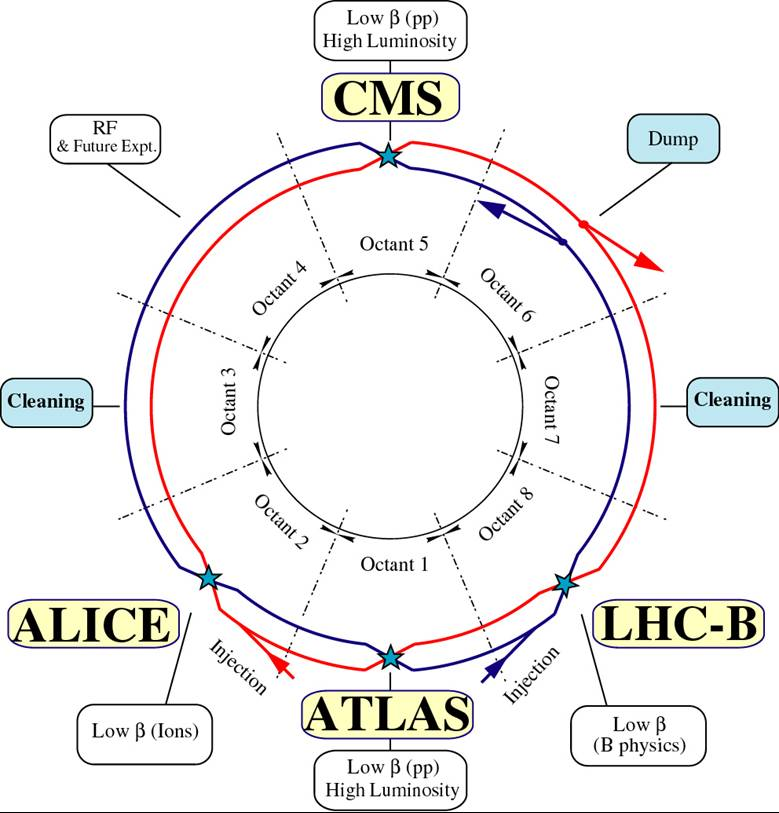
\includegraphics[width=0.7\textwidth]{img/I-2-lhc/lhc.jpg}
		\caption{Schematic representation of the Large Hadron Collider complex under the Franco-Swiss border detailling the location of the four experiment (ALICE, ATLAS, CMS, and LHCb) that analyze the produced collision [CERN].}
		\label{fig:I-2-lhc-schematic}
	\end{figure}

  The LHC's construction was approved by the CERN Council in December 1994 and started in 1998 by the excavation of the caverns that would hold the experiment sites. In 2003, the first section of the accelerator was assembled inside the tunnel and assembly continued until 2008 when the last piece was mounted and the LHC was complete and ready to produce its first collisions. After a successful preliminary run in August of the same year, an incident occurred shutting down the machine for nearly a year. Between 2010 and 2012, the accelerator has been operated at an energy of 8 TeV before shutting down for a technical Long-Shutdown (LS), a maintainance periode that allows 

  Since then, the LHC has slowly been ramping up the energy of the collisions, reaching a record breaking 14 TeV in the center of mass reference frame.

  \section{Injection Complex}

		Before being accelerated and collided by the LHC, the protons and ions are produced and sped up by multiple accelerators. Figure \ref{fig:lhc_and_cms__lhc_injection_chain} depicts the injection chain of the LHC. The first element in this chain is the \emph{Linac2}, which produces protons by ionizing gaseous hydrogen. These protons are accelerated and regrouped into bunches by a set of magnets before being transferred to the \emph{Proton Synchrotron Booster} (Booster), \emph{Proton Synchrotron} (PS), and \emph{Super Proton Synchrotron} (SPS), which furthermore increase the bunches' energy. Finally, the particles enter the LHC through two different tubes traveling in opposite directions.

		\begin{figure}[h!]
			\centering
			% 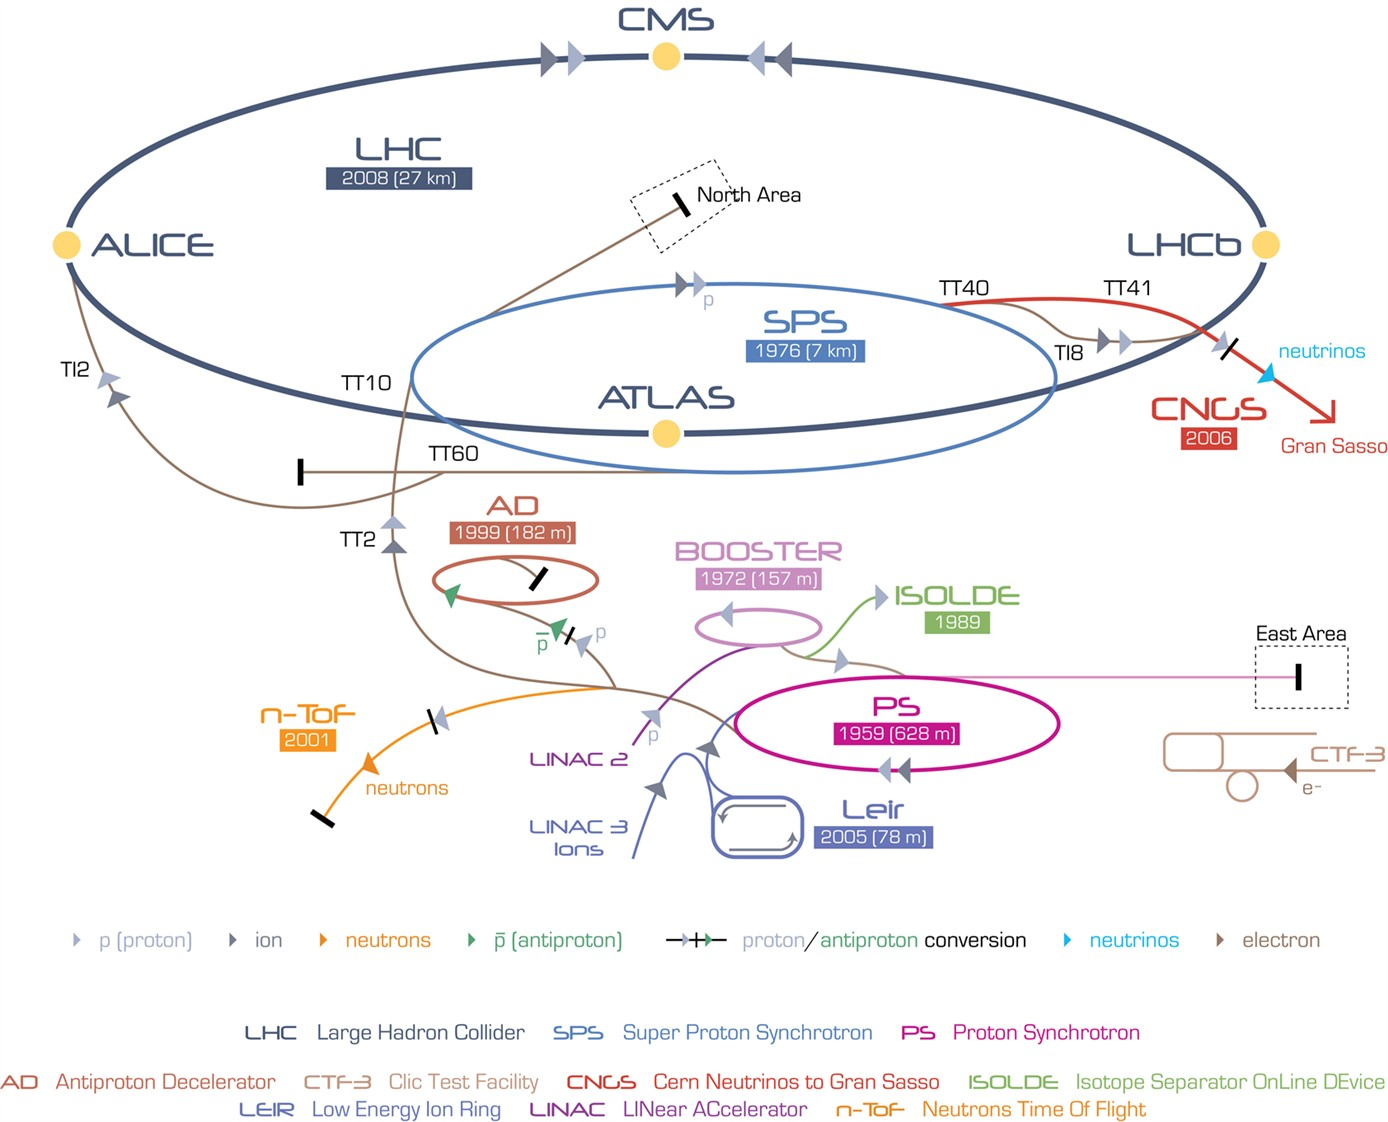
\includegraphics[width = 12cm]{2_LHC_CMS/img/lhc_injectors.jpg}
			\caption{Schematic representation of the LHC's injection chain composed of multiple smaller accelerators \Cite{Fig_LHC_Chain}.}
			\label{fig:lhc_and_cms__lhc_injection_chain}
		\end{figure}

	\section{Preformance Goals}

  	As previously mentioned, the particle beam is not a continuous flux of protons but rather a series of bunches that travel along the tube and are accelerated, regrouped, and focused by a set of magnets. Once they achieve the desired energy they are collided at a frequency of 40 MHz at the four crossing sites. \\

  	The LHC also delivers a high instantaneous luminosity $ \mathcal{L} $ which is essential to detect rare processes as it yields the apparition's frequency of events in a given interaction process
  	\begin{equation}
  		f_{process} = \mathcal{L} \sigma_{process} \ ,
  	\end{equation}
  	where $ f_{process} $ is the number of expected events per second, and $ \sigma_{process} $ is the interaction cross-section of the process. For a circular collider, the instantaneous luminosity is defined as
  	\begin{equation}
  		\mathcal{L} = \frac{N^2_b n_b f_{rev} \gamma}{4 \pi \epsilon_n \beta^*} F \ ,
  		\label{eq:lhc_and_cms__luminosity}
  	\end{equation}
  	where $ N_b $ is the number of protons or ions per bunch, $ n_b $ is the number of bunches per beam, $ f_{rev} $ is the revolution frequency, $ \gamma $ is the Lorentz factor, $ \epsilon_n $ is the beam emittance, $ \beta^* $ is the beta function at the \emph{Interaction Point} (IP), and $ F $ is a function of the crossing angle between the beams at the IP. The $ \epsilon_n $ and $ F $ parameters are related to the bunches' structure and more specifically to their spatial spreading. These parameters change during the machine's operation as the number of protons per bunch decreases, and the bunches spread out. We can integrate $ \mathcal{L} $ over a long period of time in order to get the integrated luminosity
  	\begin{equation}
  		L = \int \mathcal{L} \ dt \ ,
  	\end{equation}
  	which results in the number of events we can expect for a given interaction process
  	\begin{equation}
  		N_{process} = L \sigma_{process} \ .
  		\label{eq:lhc_and_cms__luminosity_to_N}
  	\end{equation}

	\section{Operations and Schedule}

		The LHC's operation plan \Cite{CMS_Upgrades} is divided in two phases: phase 1 during which the machine will slowly reach its nominal capabilities, and phase 2 where the machine will run at even higher luminosity after undergoing a major upgrade. \\

		Phase 1 extends from 2010 to about 2020 and is divided into three shorter periods separated by two Long Shutdowns. Table \ref{tab:lhc_and_cms__lhc_performances} shows the energy and luminosity at which the LHC will be running after both maintenances (LS1 and LS2). While the machine is shut down, physicists will have access to the detectors and will be able to perform repairs and upgrades. \\

		\begin{table}[h!]
			\centering
			\begin{tabular}{l|c|c}
				Period & Energy & Luminosity \\ \hline
				2010-2012 & 7-8 TeV & 0.5 10$ ^{34} $ cm$ ^{-2} $ s$ ^{-1} $ \\
				Long Shutdown 1 (LS1) & - & - \\
				2015-2017 & 13-14 TeV & 10$ ^{34} $ cm$ ^{-2} $ s$ ^{-1} $ \\
				Long Shutdown 2 (LS2) & - & - \\
				2019-2021 & 14 TeV & 2 10$ ^{34} $ cm$ ^{-2} $ s$ ^{-1} $
			\end{tabular}
			\caption{Energy and luminosity of the LHC during the different periods of phase 1 \Cite{LHC_Machine}.}
			\label{tab:lhc_and_cms__lhc_performances}
		\end{table}

		After LS1, the energy will be increased by using the magnets at full capability, and the luminosity will be multiplied by a factor of two by bringing down the time between two collisions to 25 ns instead of 50 ns. The luminosity will further be increased after LS2 when the machine enters the \emph{High Luminosity LHC} (HL-LHC) era. As reviewed in Equation \ref{eq:lhc_and_cms__luminosity}, various parameters can be tuned in order to achieve that goal. The main possibilities are to \Cite{LHC_LS1, LHC_Upgrade_Scenarios}
		\begin{enumerate}
			\item increase the number of bunches $ \sim n_b $;
			\item increase the number of protons per bunch by making them longer $ \sim N_b $;
			\item increase the collisions' frequency $ \sim f_{rev} $;
			\item decrease the bunches' spread by improving the efficiency of the focusing magnets $ \sim \epsilon_n $;
			\item decrease the collisions' angle by adding magnets near the IPs $ \sim F $. \\
		\end{enumerate}

		Phase 2 involves a major upgrade of the LHC and of the injection chain which would occur during LS3 after 2021. The objective is to increase the luminosity by a factor of 10 to reach 10$ ^{35} $ cm$ ^{-2} $ s$ ^{-1} $.
